\documentclass[14pt, a4paper]{article}

\usepackage{amssymb}
\usepackage{extsizes}
\usepackage{graphicx}
\usepackage{xcolor}
\usepackage{caption}
\usepackage{listings}
\usepackage{tabularx}
\usepackage{indentfirst}
\usepackage[T2A]{fontenc}
\usepackage[utf8]{inputenc}
\usepackage[english,russian]{babel}
\usepackage[left=30mm, right=10mm, top=20mm, bottom=20mm]{geometry}
\usepackage{ucs}

\graphicspath{{images/}}

\linespread{1.3}
\setcounter{tocdepth}{4}
\setlength{\parskip}{1.5pt}

\begin{document}	
	\section*{Продолжение предыдущей лекции}
	
	В 1964 году MIT создал ОС CTSS (Compatible Time Sharing System) для IBM7094. Терминалы подключались через телефонные сети. Идея оказалась удачной и получила дальнейшее развитие.
	
	В 1965 году появилась ОС Multics (Multiplexed Information and Computing Service). К разработке подключилась Bell Lab.
	
	С 1963 года D. Ritchie являлся частью Bell Lab (работал над MAC (Multiple Access Computer)), а позже - (BTL (Bell Telephone Lab)), где занимался созданием системы разделения времени для GE 645.
	
	Multics сразу являлась системой разделения времени.
	
	1969 год - Bell отделяется от работы над Multics.
	
	Томпсон, Ритчи и [...] продолжают работы, но им требуется более мощная система. Они останавливаются на PDP-7 и CrossASM GE. Томпсон начинает писать свою ОС под PDP-7 и начал он с файловой подсистемы. {\bf Это стало началом UNICS (UNIX).}
	
	Потребовался новый язык высокого уровня - B. Но в B не было типов, и он был интерпретируемым. Поэтому начали писать C, который стал компилируемым и приобрел такой тип данных как структуры (как и типы, собственно). {\bf Язык C был использован для написания UNIX.}
	
	\subsection*{Четвертое поколение}
	
	Ознаменовалось появлением больших интегральных схем (сейчас существуют сверхбольшие интегральные схемы).
	
	Современные процессоры - программно управляемые устройства (под управлением [...]). При этом сязка ЦП-ОЗУ до сих пор компьютер.
	
	\section*{Дисциплина курса}
	
	\begin{itemize}
		\item управление процессорами;
		
		\item управление памятью;
		
		\item управление данными;
		
		\item управление внешними устройствами;
		
		\item взаимодействие с процессами;
	\end{itemize}

	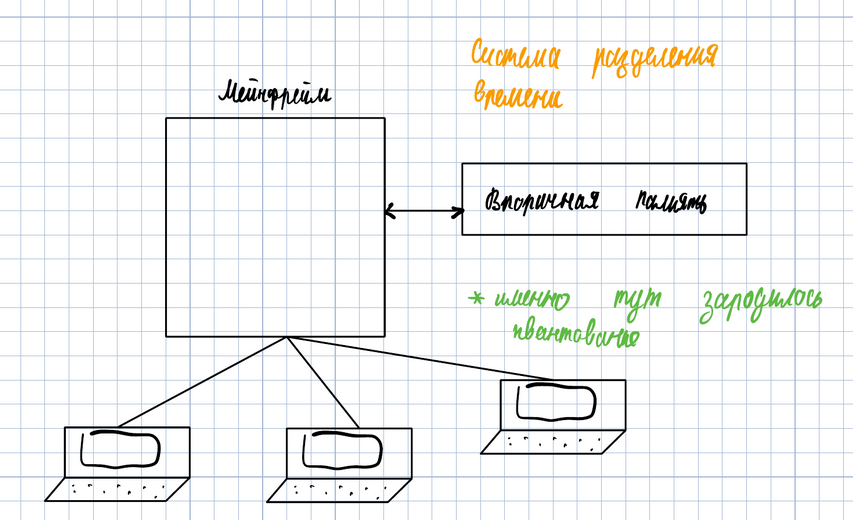
\includegraphics[width=\linewidth]{1}
	
	\subsection*{Терминалы}
\end{document}
